\documentclass[letterpaper,12pt]{article}

\usepackage{tabularx} % extra features for tabular environment
\usepackage{amsmath}  % improve math presentation
\usepackage{amssymb}
\usepackage{multirow}
\usepackage{xcolor}
\usepackage{gensymb}
\usepackage{appendix}
\usepackage{bigints}
\usepackage{mathtools}
\usepackage{gensymb}
\usepackage{float}
\usepackage{listings}
\usepackage[export]{adjustbox}
\usepackage[super]{nth}
\usepackage{graphicx} % takes care of graphic including machinery
\usepackage[margin=1in,letterpaper]{geometry} % decreases margins
\usepackage{cite} % takes care of citations
\usepackage[final]{hyperref} % adds hyper links inside the generated pdf file
\newcommand*{\tran}{^{\mkern-1.5mu\mathsf{T}}}
\DeclarePairedDelimiter\ceil{\lceil}{\rceil}
\DeclarePairedDelimiter\floor{\lfloor}{\rfloor}
\hypersetup{
    colorlinks=false,       % false: boxed links; true: colored links
    linkcolor=blue,        % color of internal links
    citecolor=blue,        % color of links to bibliography
    filecolor=magenta,     % color of file links
    urlcolor=blue         
}
%++++++++++++++++++++++++++++++++++++++++++++++++++++++++++++++++++++++++++++++++



%++++++++++++++++++++++++++++++++++++++++++++++++++++++++++++++++++++++++++++++++
% Start modifying the labwork number, your team number and the name and METU id
% of your group members.
\newcommand{\reporttitle}{Solution Set 6}
\newcommand{\reportauthor}{ Volkan Aydıngül (Id: 0075359 )\\
                            }
                            % If any teammate does not help to write this report,
                            % you may not write his/her name here.
%++++++++++++++++++++++++++++++++++++++++++++++++++++++++++++++++++++++++++++++++



%++++++++++++++++++++++++++++++++++++++++++++++++++++++++++++++++++++++++++++++++
% DO NOT MODIFY THIS SECTION
\begin{document}
\begin{titlepage}
\newcommand{\HRule}{\rule{0.7\linewidth}{0.5mm}}
\begin{center} % Center remainder of the page
%	LOGO SECTION

\includegraphics[width = 8cm]{figures/koc_logo.png}

%	HEADING SECTIONS
\textsc{\Large PHYS 514 - Computational Physics}\\[1.5cm] 
%	TITLE SECTION
\HRule \\[0.6cm]
{ \huge \bfseries \reporttitle}\\ % Title of your document
\HRule \\[1.5cm]
\end{center}
\vspace{2cm}
%	AUTHOR SECTION
\begin{flushleft} \large
\textit{Author:}\\
\reportauthor% Your name
\end{flushleft}
\vspace{2cm}
\makeatletter
Date: \@date 
\vfill % Fill the rest of the page with whitespace
\makeatother
\end{titlepage}
%++++++++++++++++++++++++++++++++++++++++++++++++++++++++++++++++++++++++++++++++




\tableofcontents
\newpage





%\begin{figure}[H] 
%   \centering \includegraphics[width=\columnwidth]{figures/figure.png}           
%                \caption{Caption}                
%                   \label{fig:label}
%   \end{figure}

\section{Problem XVIII}
\subsection{Problem Definition}
\paragraph{} In this problem, the aim is to find a curve-physical path- that yields the minimum time when an object travel through it under gravity. This problem, in mathematical terms, can be defined as follows: Find the function $f(x)$ that minimizes the below relation.

\begin{equation}
    \int_{x_0}^{x_f} \sqrt{\frac{1 + \left(\frac{dy}{dx}\right)^2}{2gy}}dx
    \label{eq:brach}
\end{equation}
\paragraph{}In above equation, numerator represents the length of the path that is charactarized by the $f(x)$, while denominator represents the instantaneous velocity of the moving object at given $y$ value.

\subsection{Genetic Algorithm}
\paragraph{}In the \textit{Genetic Algorithm}, the main idea is to solve an optimization problem via inspiring by the evolutionary principles that one might encounter in the pure nature. With the simplest terms, the genetic algorithm can be recognized from three steps. Below, these three steps will be discussed.

\subsection{Model Initialization}
\paragraph{} In model initialization, basically, the sample space that represents the population of candidate solutions is created. Every individual in the population corresponds to a one candidate solution. Also, every individual has its own genetic information, namely, one can say DNA, or chromosomes and etc. The initial values stored in the DNA can be chosen via random declaration or a systematic approach. The evolution of the information stored in the DNA will determine the faith of the algortihm, namely, the solution.

\subsection{Selection}
\paragraph{} In this part, the main principle is to measure how well the individuals are able to survive for a given environment, that is, the initial condition. How well the each individual can survive is determined based on the predetermined \textit{objective function}. The objective function selection can vary depending on the problem. In this problem, the objective function can be defined as the discritisized version of the \eqref{eq:brach}. For a given $x_0$ - $x_f$ interval, one can, for instance, randomly assign $y_i$ values, then, to evaluate the \eqref{eq:brach} is nothing but the numerical differentiation and integration. Finally, one should contructa an entity called mating pool. The basic idea behind the mating pool is to collect the most promising individuals and perform reproduction between them. Surely, it is not a good ideo to completely eliminate to unpromising individuals, because they can also carry information, that is useful, in their DNA. Therefore, the more suitable methodology is to construct mating pool by sampling based on a previously calculated probalilities. In this problem, the sampling probability can be defined as follows:
\begin{itemize}
    \item Calculate fitness of each individual.
    \item Since it is a minimization problem, take inverse and square of each element to represent fittest element as having the highest numerical value.
    \item Apply $softmax$ operator to the generation to calculate probablilities.
\end{itemize}
where $softmax$ operator can be defined as following:

\begin{equation*}
    softmax(\vec{x}) = \frac{e^{x_i}}{\sum e^{x_i}}
\end{equation*}

\paragraph{} In this calculation scheme, finally, the mating pool would be constructed such that the fittest individuals are probabilistically the frequent ones.
\subsection{Reproduction}
\paragraph{} Finally, in the reproduction phase, the main idea is to create an interaction between the individuals displaying different properties so as to create a new generation wihch might have fitter individuals. The reproduction scheme can be defined in many ways, but, the simples one is to reunite the different proportions of two given individual DNAs. In addition, to be able to mimic nature accurately, one further operation might be \textit{mutation}. As can be inferred from the nature itself, the mutation can be defined as the arbitrary alteration of the elements of the DNA. It, in the end, helps model to get rid of the stucked undesired properties.

\paragraph{} As a final note, one can easily conclude that this inspiring algorithm is haighly dependent on the hyperparameters such as population size, DNA size, mutation rate, and number of generations. 

\subsection{Sad Note :(}
\paragraph{} \emph{Although I explained the steps I took to construct genetic algorithm, unfortunately, I got stuck somewhere and could not achieve to produce reasonable results.}
\section{Problem XVIV}
\subsection{Nondimensialization of the Two-Body Problem}
\paragraph{} The differential equation that defines the two body problem can be observed below:

\begin{equation*}
    m_i \frac{d^2 \vec{r_i}}{dt^2} = -\frac{G m_1 m_2}{\lvert \vec{r_1} + \vec{r_2}  \rvert} \hat{r_i}
\end{equation*}

\paragraph{} It is always better to define equations in a nondimensional format, because it helps to reduce the difficulties that might be a result of order of magnitude of the dependent and independent variables. The common approach to this problem is to scale variable with a common magnitude. Firstly, the common magnitudes should be defined for each variable. To be able to scale distance, the $r_p$ (the distance between Jupiter and Sun at perihelion) is good a choice. Then, the nondimensional distance can be defined as follows:

\begin{equation*}
    \rho_i = \frac{r_i}{r_p}
\end{equation*}

\paragraph{} In the same way, the time can be nondimensionalized via using a common term. This term can be the period of their orbit propogation. From the \textit{Kepler's $3_{rd}$ Law}, it can be defined that:

\begin{equation*}
    t_0 = \sqrt{\frac{r_p^3}{G\left(m_J + m_S\right)}}
\end{equation*}

where $m_S$ and $m_J$ are masses of Jupiter and Sun, respectively. Then, the nondimensionalized time can be defined as follows:

\begin{equation*}
    \tau = \frac{t}{t_0}
\end{equation*}

\paragraph{} For the case of mass, the reduced mass can be defined as:

\begin{equation*}
    \mu = \frac{m_J m_S}{m_J + m_S}
\end{equation*}

Then, the nondimensionalized form of the mass is as follows:

\begin{equation*}
    \mu_i  = \frac{m_i}{\mu}
\end{equation*}

\paragraph{} Now, it is time to transform differential term. Firstly, it is obvious that:
\begin{equation*}
    d^2\vec{r_i} = d^2\vec{\rho_i} r_p 
\end{equation*}

However, the time differential is not as obvious as displacement. The following relation must be constructed:

\begin{equation*}
    \frac{d}{dt} = \frac{d\tau}{dt}\frac{d}{d\tau} = \frac{1}{t_0} \frac{d}{d\tau}
\end{equation*}

If one executes the above operation recursively, finally, the following relation could be hold:

\begin{equation*}
    \left( \frac{d}{dt} \right) ^n = \frac{1}{t_0^n} \frac{d^n}{d\tau^n}
\end{equation*}

From here, one can conclude that:

\begin{equation*}
    \frac{d^2\vec{r_i}}{dt^2} = \frac{d^2\rho}{d\tau^2} \frac{r_p}{t_0^2} =  \frac{d^2\rho}{d\tau^2} \frac{r_p G \left(m_1 + m_2\right)}{r_p^3}
\end{equation*}

\paragraph{} Now, it is time to plug all values with its nondimensionalized form.

\begin{equation*}
    \frac{\mu_i \left(m_1  m_2\right)}{m_1 + m_2} \frac{d^2\rho}{d\tau^2} \frac{r_p G \left(m_1 + m_2\right)}{r_p^3} = -\frac{G \left(m_1 + m_2\right)}{\lvert \vec{\rho_1} + \vec{\rho_2} \rvert^2 {r_p^2}}\hat{\rho_i}
\end{equation*}

\paragraph{} Finally, cancellation of related terms yields the following:

\begin{equation*}
    \mu_i \frac{d^2 \vec{\rho_i}}{d\tau^2} = - \frac{1}{\lvert \vec{\rho_1} + \vec{\rho_2} \rvert^2} \hat{\rho_i}
\end{equation*}


\subsection{Orbit Propagation}
\paragraph{} When the Figure \ref{fig:10}, \ref{fig:11}, \ref{fig:12}, and \ref{fig:13} are observed, it can be observed that as the timestep decreases, the orbits become a perfect ellipse, which is coherent with the theory and analytical solution. However, in Figure \ref{fig:10}, it can be also observed that, even if the timestep is relatively high compared to the lower ones, still, \textit{Runge Kutta 4} and \textit{Symptactic Euler} method manages to preserve its ellipse shape. Because, these two method, especially Symptactic Euler, are tended to preserve the energy in the system 
\begin{figure}[H]
    \centerline{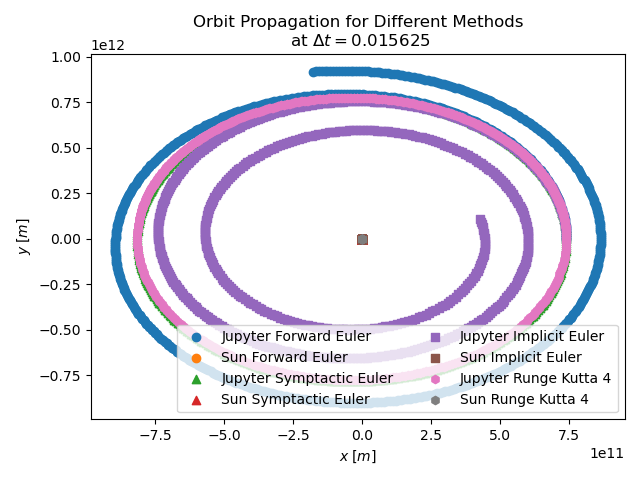
\includegraphics[width=0.7\linewidth]{figures/10.png}}
    \caption{Orbit Propagation of Different Methods at $\Delta t = 2^{-6}$}
    \label{fig:10}
    \end{figure}
    
\paragraph{} In Figure \ref{fig:11} and Figure \ref{fig:12}, the correction on the orbits can be observed, however, there are still some discrepancies in the orbit.
    \begin{figure}[H]
    \centerline{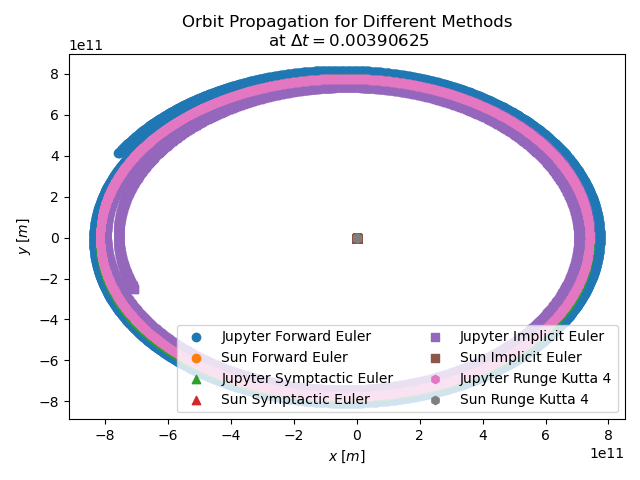
\includegraphics[width=0.7\linewidth]{figures/11.png}}
    \caption{Orbit Propagation of Different Methods at $\Delta t = 2^{-8}$}
    \label{fig:11}
    \end{figure}
    \begin{figure}[H]
    \centerline{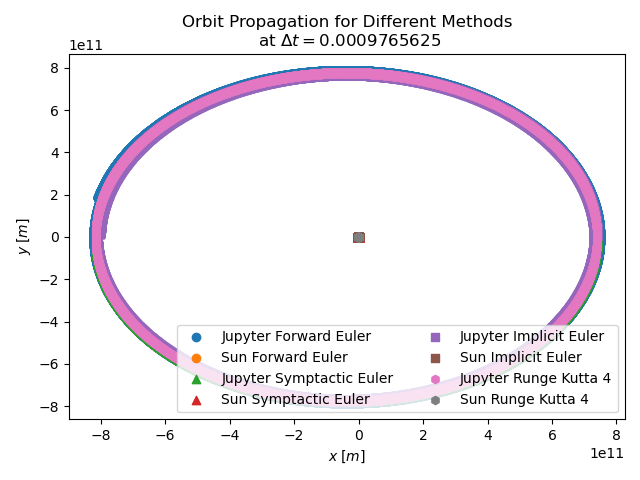
\includegraphics[width=0.7\linewidth]{figures/12.png}}
    \caption{Orbit Propagation of Different Methods at $\Delta t = 2^{-10}$}
    \label{fig:12}
    \end{figure}
\paragraph{} In Figure \ref{fig:13}, the perfection of the ellipse orbit can be observed.
    \begin{figure}[H]
    \centerline{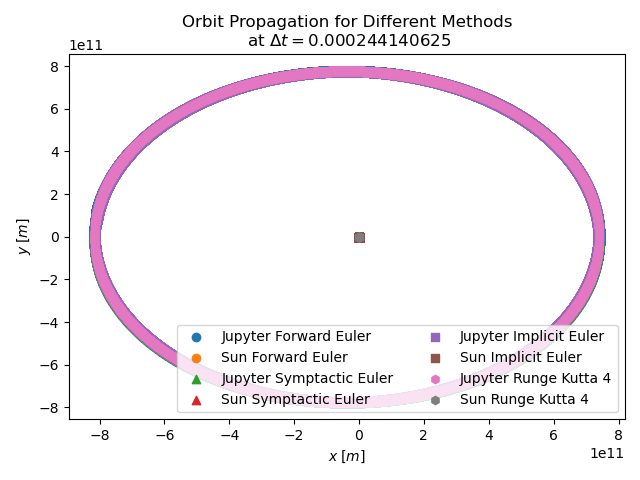
\includegraphics[width=0.7\linewidth]{figures/13.png}}
    \caption{Orbit Propagation of Different Methods at $\Delta t = 2^{-12}$}
    \label{fig:13}
    \end{figure}
\label{sec:orbit}
\subsection{Angular Momentum}  

\paragraph{} Actually, from now on, the similar discussion held on the \ref{sec:orbit} can be applicable for upcoming sections. In Figure \ref{fig:20}, \ref{fig:21}, \ref{fig:22}, and \ref{fig:23}, it can be inferred that, as mentioned previously, the Symptactic Euler method and Runge Kutta 4 method are tended to preserve the characterisctics of the system. Therefore, in all of the aforamentioned figures, the red-square and orange-triangle curves stand idle.  
    \begin{figure}[H]
    \centerline{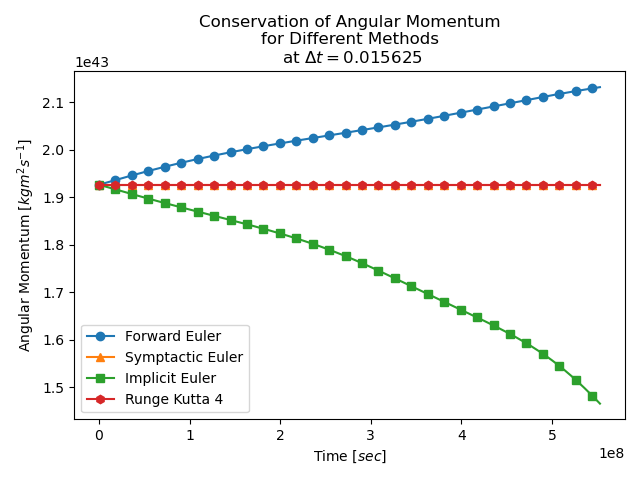
\includegraphics[width=0.7\linewidth]{figures/20.png}}
    \caption{Total Angular Momentum of Planets at $\Delta t = 2^{-6}$}
    \label{fig:20}
    \end{figure}
    
    \begin{figure}[H]
    \centerline{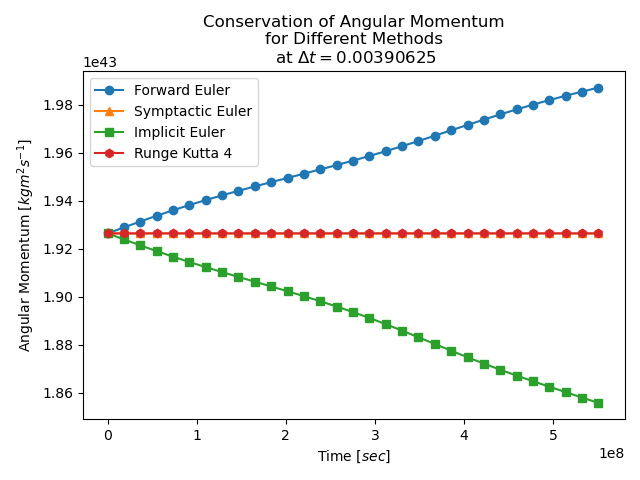
\includegraphics[width=0.7\linewidth]{figures/21.png}}
    \caption{Total Angular Momentum of Planets at $\Delta t = 2^{-8}$}
    \label{fig:21}
    \end{figure}
\paragraph{}However, as can be inferred from Figure \ref{fig:20}, \ref{fig:21}, \ref{fig:22}, and \ref{fig:23}, the \textit{Forward Euler} and \textit{Implicit Euler} method could not conserve the angular momentum.
    \begin{figure}[H]
    \centerline{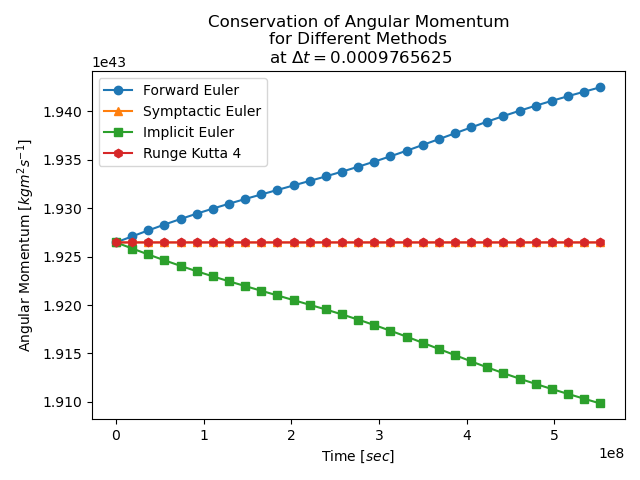
\includegraphics[width=0.7\linewidth]{figures/22.png}}
    \caption{Total Angular Momentum of Planets at $\Delta t = 2^{-10}$}
    \label{fig:22}
    \end{figure}
    
    \begin{figure}[H]
    \centerline{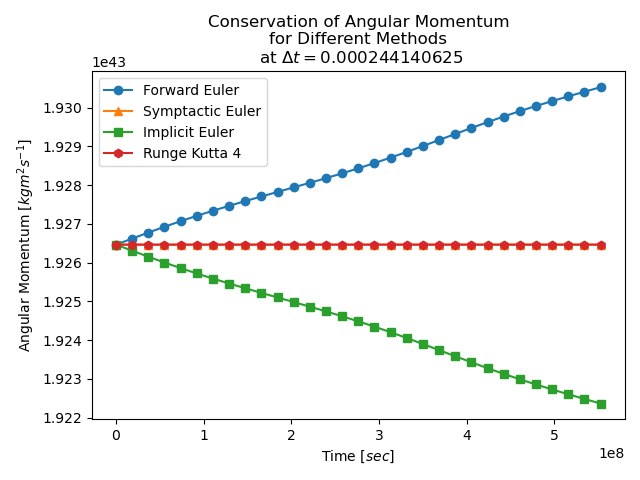
\includegraphics[width=0.7\linewidth]{figures/23.png}}
    \caption{Total Angular Momentum of Planets at $\Delta t = 2^{-12}$}
    \label{fig:23}
    \end{figure}

\subsection{Linear Momentum}
\paragraph{}From Figure \ref{fig:30}, \ref{fig:31}, \ref{fig:32}, and \ref{fig:33}, it can be investigated that the linear momentum profile of the orbit propagation of the planets has a highly fluctuating structure.
    \begin{figure}[H]
    \centerline{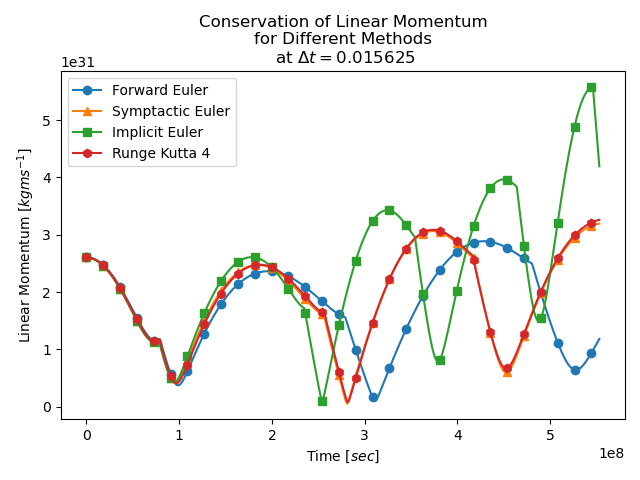
\includegraphics[width=0.7\linewidth]{figures/30.png}}
    \caption{Total Linear Momentum of Planets at $\Delta t = 2^{-6}$}
    \label{fig:30}
    \end{figure}
\paragraph{} However, it can be also observed that as the timestep decreases, all the curves are starting to conincide with red and orange curve, which belongs to the Symptactic Euler and Runge Kutta 4 method.
    \begin{figure}[H]
    \centerline{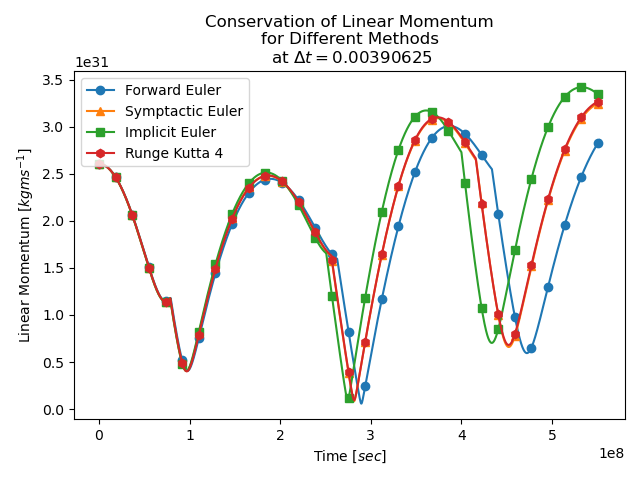
\includegraphics[width=0.7\linewidth]{figures/31.png}}
    \caption{Total Linear Momentum of Planets at $\Delta t = 2^{-8}$}
    \label{fig:31}
    \end{figure}
\paragraph{} From this investigation, one more time, the preservative structure of the Symptactic Euler and Runge Kutta 4 method can be admired. 
    \begin{figure}[H]
    \centerline{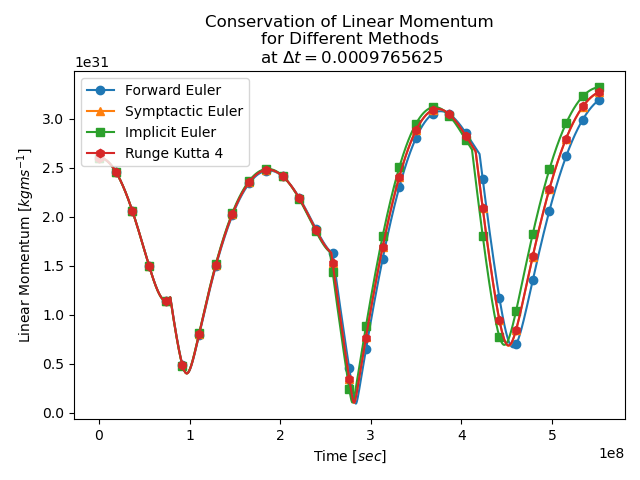
\includegraphics[width=0.6\linewidth]{figures/32.png}}
    \caption{Total Linear Momentum of Planets at $\Delta t = 2^{-10}$}
    \label{fig:32}
    \end{figure}
    
    \begin{figure}[H]
    \centerline{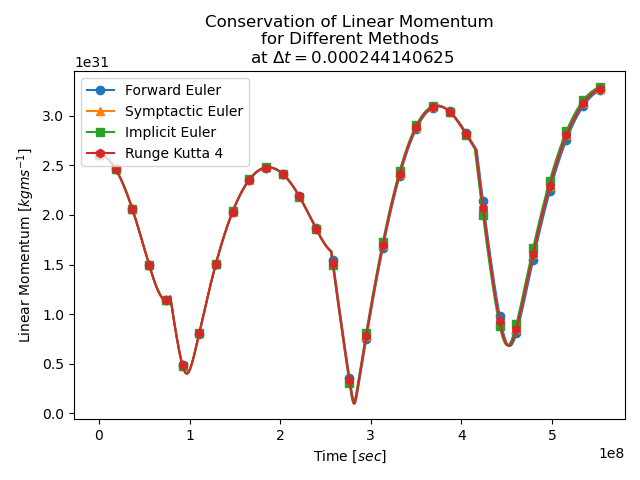
\includegraphics[width=0.7\linewidth]{figures/33.png}}
    \caption{Total Linear Momentum of Planets at $\Delta t = 2^{-12}$}
    \label{fig:33}
    \end{figure}

\subsection{Total Energy}

\paragraph{} In Figure \ref{fig:40}, \ref{fig:41}, \ref{fig:42}, and \ref{fig:43}, the change of the total energies of the planets can be observed.

    \begin{figure}[H]
    \centerline{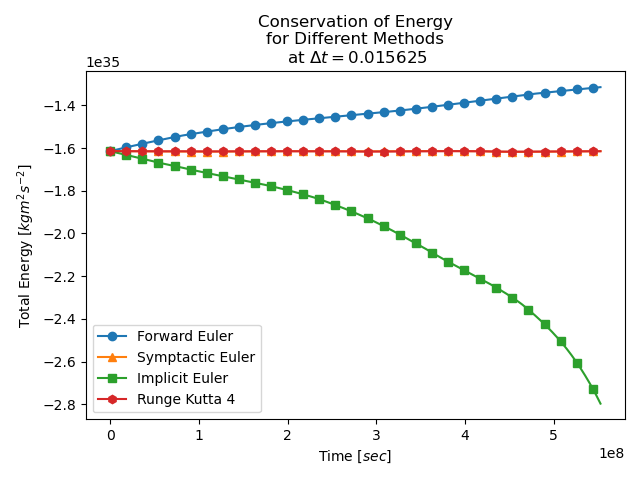
\includegraphics[width=0.7\linewidth]{figures/40.png}}
    \caption{Total Energy of Planets at $\Delta t = 2^{-6}$}
    \label{fig:40}
    \end{figure}

    \paragraph{} Investigating the total energy is, actually, a little bit different that the others. Because, unlike other quantites, the fluctuation is tended to increase as the timestep decrease.

    \begin{figure}[H]
    \centerline{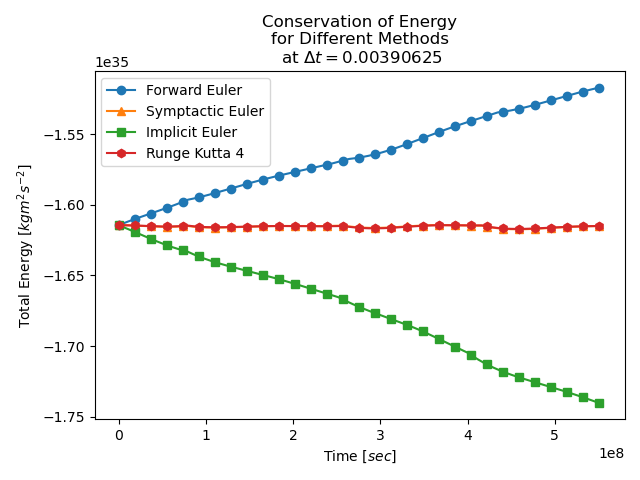
\includegraphics[width=0.7\linewidth]{figures/41.png}}
    \caption{Total Energy of Planets at $\Delta t = 2^{-8}$}
    \label{fig:41}
    \end{figure}
    \paragraph{} On the other hand, becoming a conincident curves or stable ones were not observed, as the timestep decreases, 
    \begin{figure}[H]
    \centerline{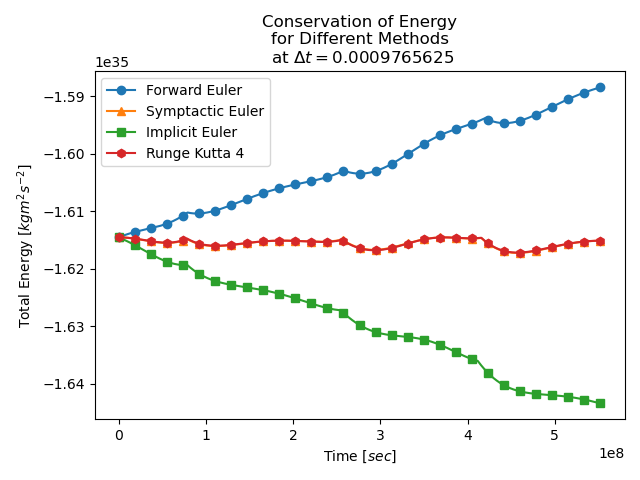
\includegraphics[width=0.7\linewidth]{figures/42.png}}
    \caption{Total Energy of Planets at $\Delta t = 2^{-10}$}
    \label{fig:42}
    \end{figure}
    
    \begin{figure}[H]
    \centerline{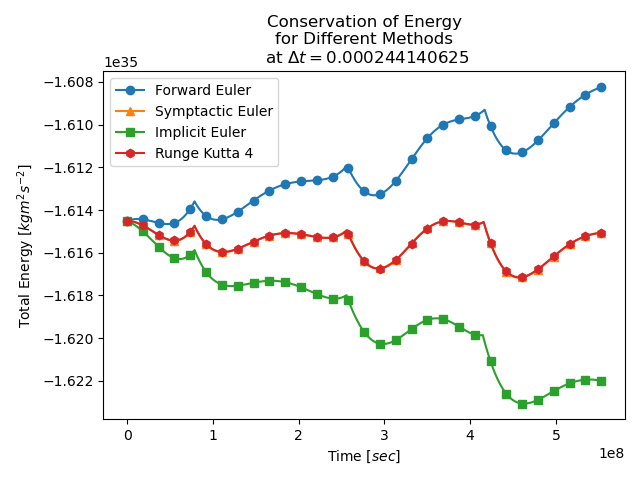
\includegraphics[width=0.7\linewidth]{figures/43.png}}
    \caption{Total Energy of Planets at $\Delta t = 2^{-12}$}
    \label{fig:43}
    \end{figure}
    
\pagebreak
\subsection{Time Comparison}

\paragraph{} From Figure \ref{fig:5}, one can clearly deduce that the fastest method is the \textit{Forward Euler} method, while the slowest one \textit{Runge Kutta 4} method. However, this speed considerations is only important when there is a computational budget. Otherwise, the more important thing is their accuracy and characteristics. Except Runge Kutta 4, all of them has a $O(h)$ error rate. However, every one of them displays different characteristics. For example, the Forward Euler method emits a fast behavior in terms of convergence and iteration, in terms of conserving dynamical quantites, it is not the best. However, as opposed to the Forward Euler method, Symptactic Euler method is superior in terms of conserving ability. One additional note might be that the slowness of  the Implicit Euler method. Its slowness comes from the fact that it solves a root-finding problem at each step to propagate differential equation.
    \begin{figure}[H]
    \centerline{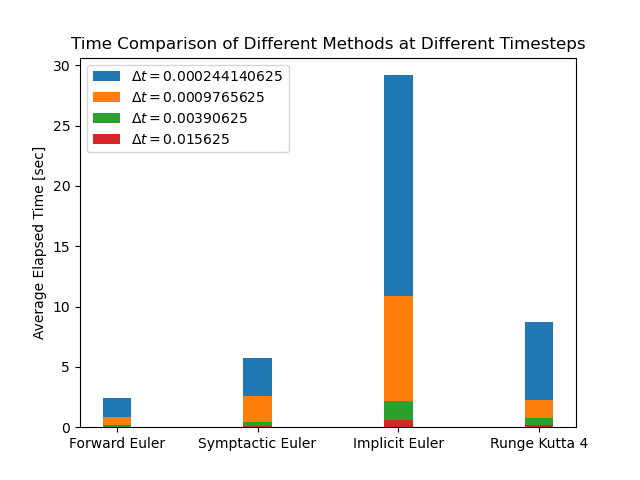
\includegraphics[width=0.9\linewidth]{figures/5.png}}
    \caption{Comparison of Elapsed Time for Different Methods at Different Timesteps}
    \label{fig:5}
    \end{figure}
    












\end{document}



              


